\documentclass[conference]{IEEEtran}
\usepackage{graphicx}
\usepackage{amsmath}
\usepackage{amssymb}
\usepackage{float}
\usepackage{subfig}
\usepackage{hyperref}
\usepackage{listings}
\usepackage{color}
\usepackage{url}
\usepackage{cite}
\usepackage{caption}
\usepackage{subfig}
\usepackage{multirow}
\usepackage{multicol}
\usepackage{booktabs}
\usepackage{tabularx}
\usepackage{array}
\usepackage{enumitem}


\begin{document}

\title{Design of Low Power 4X3 Magnitude Comparator}

\author{
\IEEEauthorblockN{Nidal Zabade}
\IEEEauthorblockA{\href{mailto:1200153@student.birzeit.edu}{1200153@student.birzeit.edu}
}
\and
\IEEEauthorblockN{Pierre Backleh}
\IEEEauthorblockA{\href{mailto:1201296@student.birzeit.edu}{1201296@student.birzeit.edu}
}
\and
\IEEEauthorblockN{Pierre Backleh}
\IEEEauthorblockA{\href{mailto:1201296@student.birzeit.edu}{1201296@student.birzeit.edu}
}
}


\maketitle

\begin{abstract}
The primary goal of this project is to design a 4x3 magnitude comparator consisting of two 2-input AND gates, three 3-input AND gates, two 4-input AND gates, two 5-input AND gates, four 2-input XOR gates, one 4-input OR gate, one 4-input XOR gate, and one transistor. In this design, the balance between low power and low delay will be taken into consideration, so we used 14nm process technology, which helps in saving power. Additionally, the Electric VLSI Design System and LT Spice tools were used to design the required circuits, including schematics, layouts, and simulations.
\end{abstract}

\begin{IEEEkeywords}

Low Power, 4X3 Magnitude Comparator, Electric VLSI Design System, LT Spice.

\end{IEEEkeywords}

\section{Introduction}

\subsection{Motivation}
The motivation behind building efficient and optimized digital comparator lies behind implementing reliable, fast, and low-power circuits that can accurately determine the relationship between binary inputs, taking into consideration the performance matrix including speed, area efficiency, power consumption, etc. 
As each chip becomes more and more complex when integrating more functionalities, it is crucially needed to implement efficient comparators, to manage and process large volumes of data quickly and accurately. Creating high-speed comparators in applications like communication systems can keep up with data rates and ensure timely decision-making, also becoming low-power can contribute to extending battery life and reducing overall energy consumption. In order to occupy the minimal silicon area in the chip while improving the performance and shrinking the size, it is needed to implement area-efficient comparator designs. These comparators also need to keep up with the technologies using semiconductors including fits and CMOS. All that can be focused on in order to optimized comparator architectures to meet the demands of the ongoing development of technology.

\subsection{Comparator Basic Function}
Comparators are a basic design module and element in modern digital VLSI design. A magnitude digital comparator is a combinational circuit that compares two digital or binary numbers to find out whether which is less than, greater than, or greater than the other number. This circuit start comparing the bits of each number starting from the Most Significant Bit (MSB) to Least Significant Bit (LSB), then when A>B output is set to one it means that A is greater, when A<B is set to one then A is less, and when A=B is set to one then A is equal to B. Comparators play a crucial role in applications, including arithmetic operations, control systems, digital signal processing, and more
\begin{figure}[h]
    \centering
    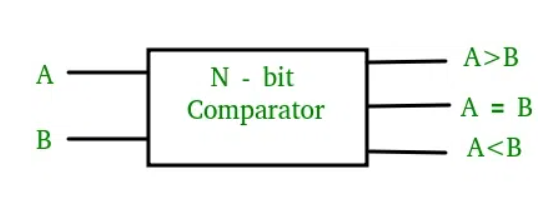
\includegraphics[width=0.3\textwidth]{assets/NbitComparator.png}
    \caption{N-bit Comparator}
    \label{fig:NbitComparator}
\end{figure}

\subsubsection{4x3 Comparator}
4x3 comparator is used to compare two binary numbers each with 4 bits. It consists of 8 inputs 4-input from each number, and three outputs indicating if equal, greater, of less than. A number consists of A0, A1, A2, A3 and B consists of B0, B1, B2, B3 which are then compared. As seen from the Figure~\ref{fig:4x3Comparator}, this comparator circuit consists of And, Nor, Or, XNOR, and invertor components.
\begin{figure}[h]
    \centering
    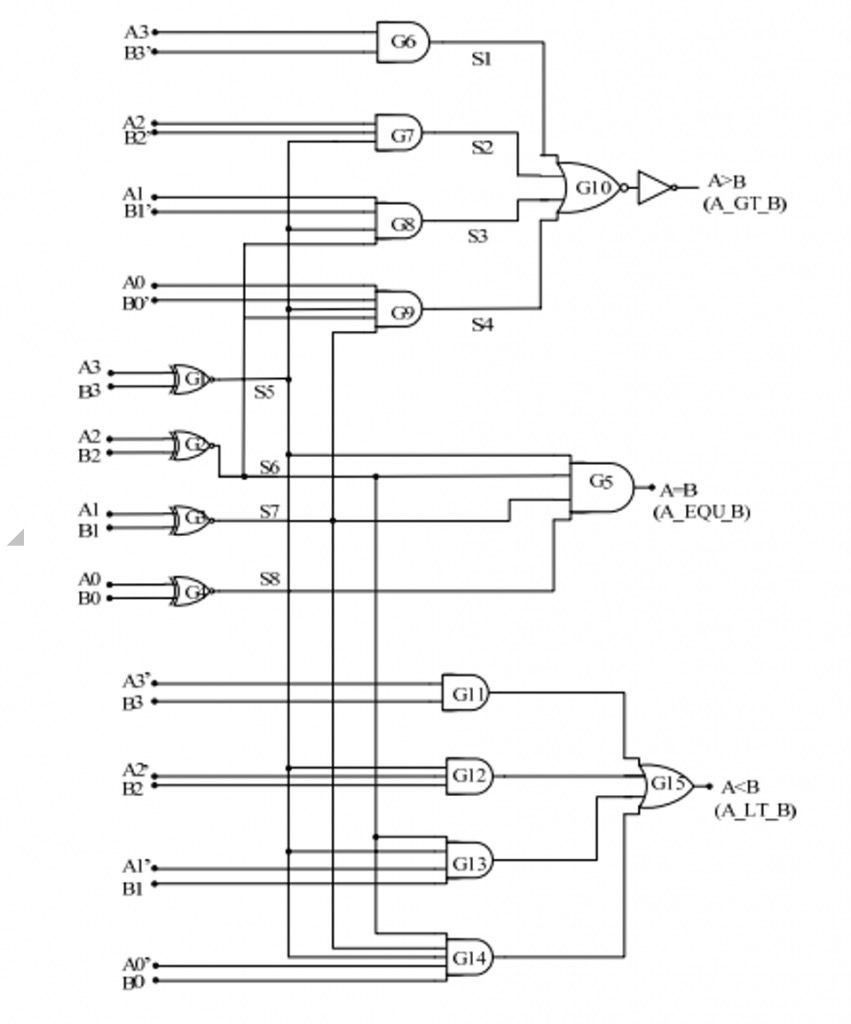
\includegraphics[width=0.3\textwidth]{assets/4x3ComparatorCircuit.jpg}
    \caption{4x3 Comparator}
    \label{fig:4x3Comparator}
\end{figure}

Figure~\ref{fig:4x3ComparatorTruthTable} shows the truth table of the 4x3 comparator, where $A>B$, $A=B$, and $A<B$ are the outputs of the comparator. The truth table shows the output of the comparator for each possible input combination.
\begin{figure}[h]
    \centering
    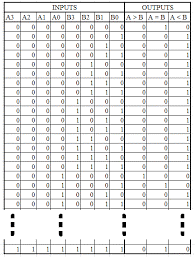
\includegraphics[width=0.3\textwidth]{assets/4x3ComparatorTruthTable.png}
    \caption{4x3 Comparator Truth Table}
    \label{fig:4x3ComparatorTruthTable}
\end{figure}

\subsubsection{4x3 Comparator Circuit Components}
In order to save area and space and minimize the propagation delay of the system, the components of the comparator circuit are built using NAND, NOR, XNOR using the PMOS and NMOS inverters. So these gates are simpler to implement in hardware compared to AND, OR, and XOR gates directly, and implementing them reduces the number of transistors required and therefore the total area consumed. They also have faster propagation delays, which can result in faster circuit response times.
\begin{itemize}
\item $A>B$ is built using a 2-input AND gate, a 3-input AND gate, a 4-input AND gate, a 5-input AND gate, and a 4-input OR gate.
\item $A=B$ is built using 2-input XOR gates, a 4-input AND gate.
\item $A<B$ is built using a 2-input AND gate, a 3-input AND gate, a 4-input AND gate, a 5-input AND gate, and a 4-input OR gate.
\end{itemize}

\subsubsection{Implement 2-input AND from NAND}
AND gate outputs 1 only when both inputs are 1, represented as \( \text{AND}(A, B) = \overline{\text{NAND}(A, B)} \)
, as can be seen from Figure~\ref{fig:ANDfromNAND} below. An AND gate can be implemented using a NAND gate composed of 2 PMOS inverters in parallel and 2 NMOS in series, followed by an inverter to obtain the AND gate functionality.
\begin{figure}[h]
    \centering
    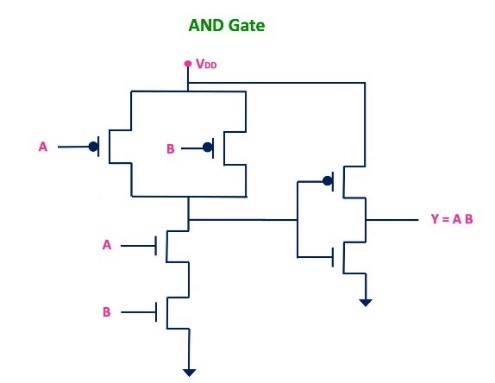
\includegraphics[width=0.25\textwidth]{assets/AndUsingNand.jpg}
    \caption{AND from NAND}
    \label{fig:ANDfromNAND}
\end{figure}
\subsubsection{Implement 3-input AND from NAND}
As described previously about the and gate logic and implementation, 3-input AND is similar as it is implemented using 3 NAND gates in series followed by an inverter

\subsubsection{Implement 4-input AND from NAND}
In order to implement a 4-input AND using two 2-input NAND gates feeding a NOR gate is used to output the same logic but enhancing the area and time consumption seen in the Figure~\ref{fig:4inputANDfromNAND} below.
\begin{figure}[h]
    \centering
    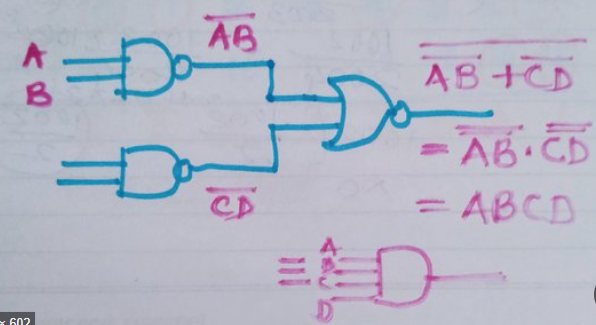
\includegraphics[width=0.25\textwidth]{assets/4inputANDfromNAND.png}
    \caption{4-input AND from NAND}
    \label{fig:4inputANDfromNAND}
\end{figure}
\subsubsection{Implement 5-input AND from NAND}
In order to implement a 5-input AND using two NAND gates, one 3-input NAND gate, and another 2-input NAND gate feeding a NOR gate are used to output the same logic but enhancing the area and time consumption.
\begin{figure}[h]
    \centering
    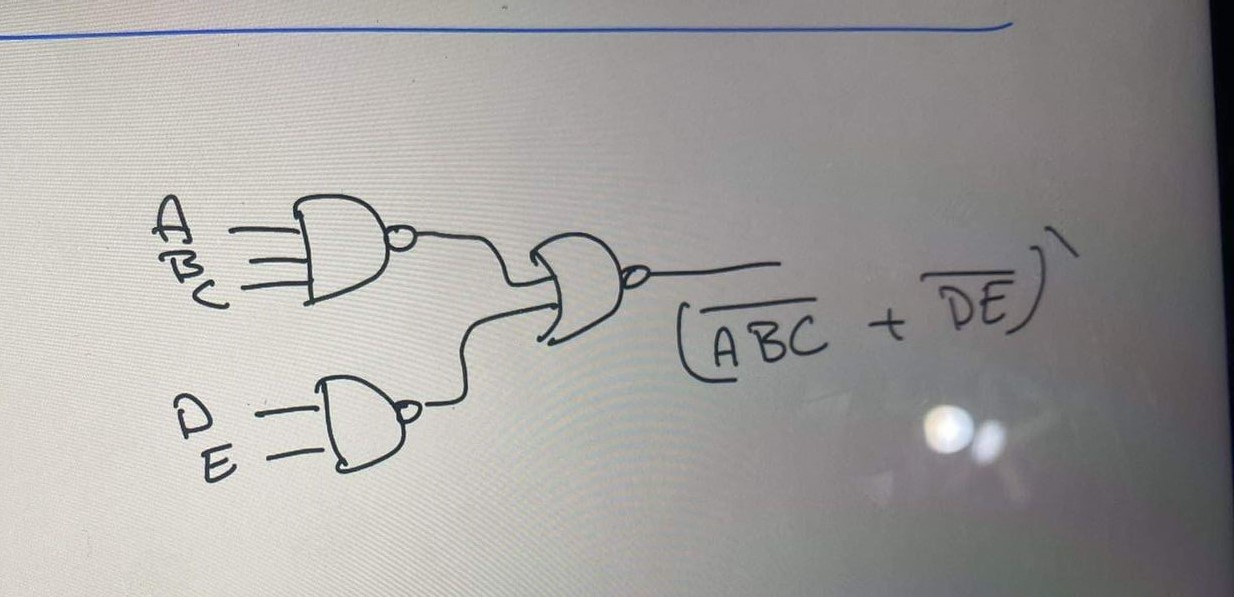
\includegraphics[width=0.25\textwidth]{assets/5inputANDfromNAND.jpg}
    \caption{5-input AND from NAND}
    \label{fig:5inputANDfromNAND}
\end{figure}
\subsubsection{Implement 2-input XNOR from NAND}
\( \text{XNOR}(A, B) = \overline{A \oplus B} \), this logic gate outputs 1 only when both inputs are the same either if 11 or 00 only. Since the NAND gate has been implemented, it can be used to efficiently implement the XNOR gate and save area and time in which each NAND gate's output feeds into the next gate as in Figure~\ref{fig:XNORfromNAND} below.
\begin{figure}[h]
    \centering
    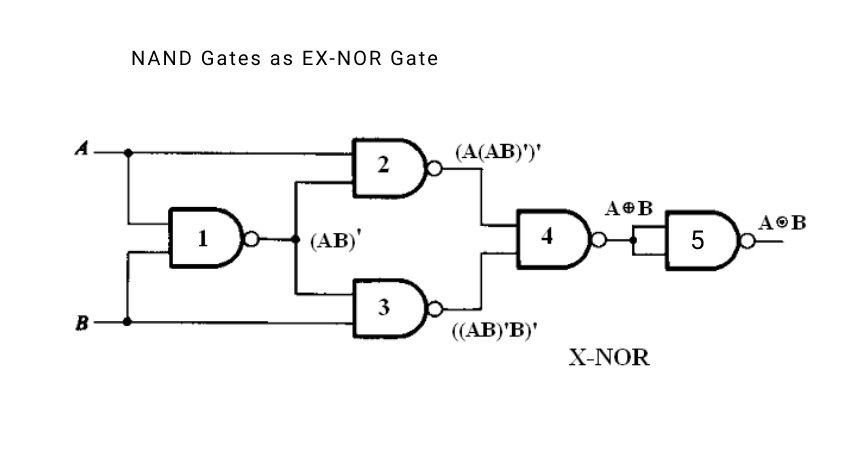
\includegraphics[width=0.25\textwidth]{assets/XNORfromNAND.jpg}
    \caption{XNOR from NAND}
    \label{fig:XNORfromNAND}
\end{figure}
\subsubsection{Implement 2-input NOR}
The NOR gate outputs 1 only when both inputs are 0, represented as \( \text{NOR}(A, B) = \overline{\text{OR}(A, B)} \), as can be seen from Figure~\ref{fig:NORCMOS} below. A NOR gate can be implemented using an OR gate composed of 2 PMOS inverters in series and 2 NMOS in parallel.
\begin{figure}[h]
    \centering
    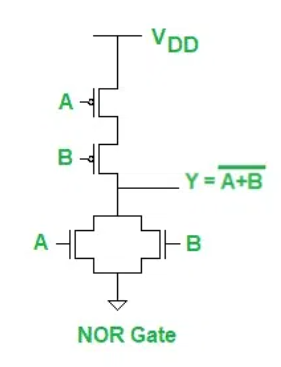
\includegraphics[width=0.2\textwidth]{assets/NORCMOS.png}
    \caption{NOR CMOS}
    \label{fig:NORCMOS}
\end{figure}

\subsubsection{Implement 4-input OR from NOR}
In order to implement a 4-input OR using two 2-input NOR gates feeding a 2-input NAND gate is used to output the same logic but enhancing the area and time consumption seen in Figure~\ref{fig:4inputORfromNORandNAND} below.
\begin{figure}[h]
    \centering
    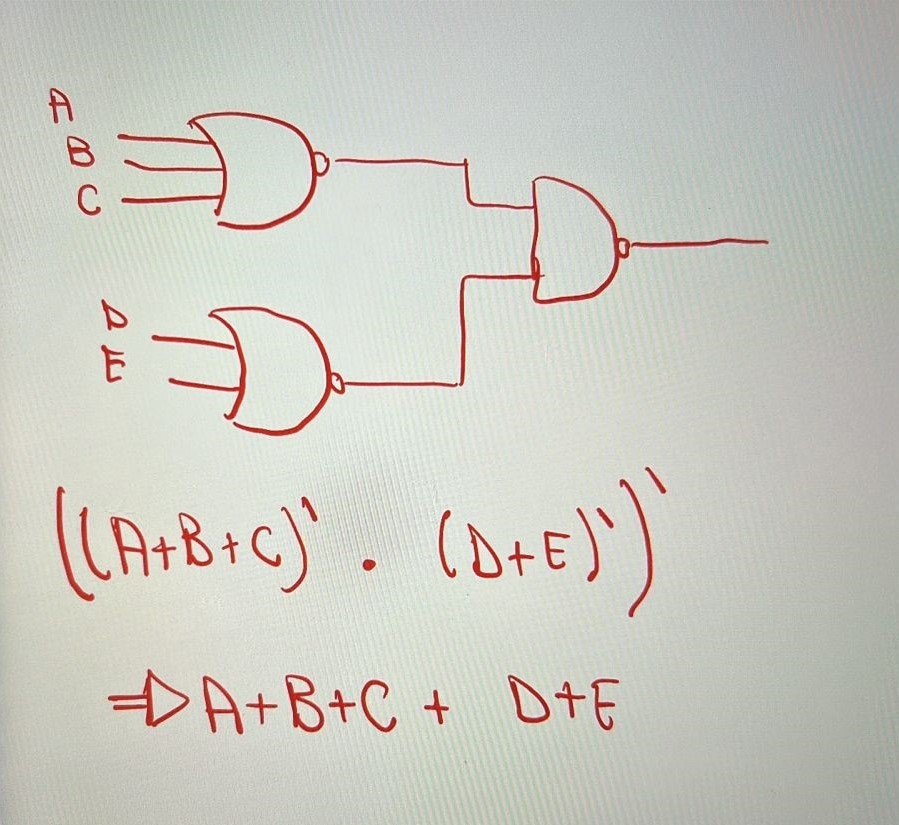
\includegraphics[width=0.25\textwidth]{assets/4inputORfromNORandNAND.jpg}
    \caption{4-input OR from NOR and NAND}
    \label{fig:4inputORfromNORandNAND}
\end{figure}


\section{Procedure, Simulations and Results}
To follow the flow of the 4-bit comparator construction, the basic circuits were built on electric binary tool as discussed in the following parts.
\subsection{Not Gate}
The inverter gate was built on the electric binary in terms of schematic, layout, and icon as shown below in Figure~\ref{fig:NotGateSchematic} and Figure~\ref{fig:NotGateLayout} respectively.
\begin{figure}[h]
    \centering
    \subfloat[Schematic of the Not Gate]{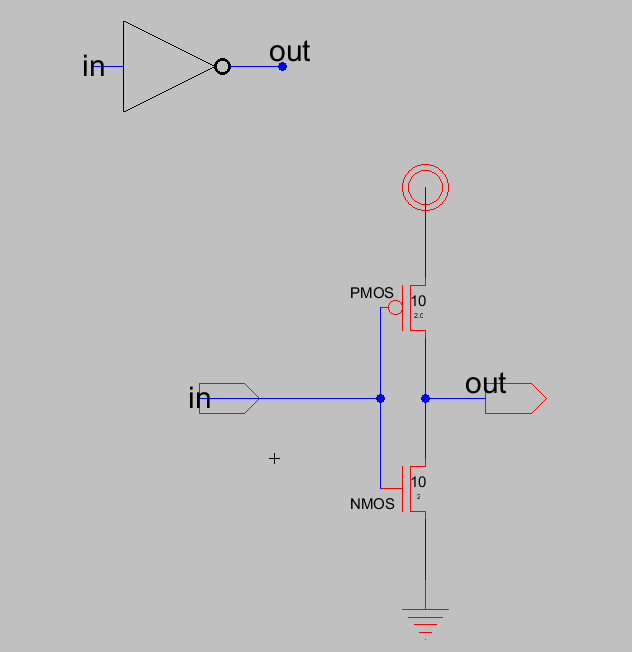
\includegraphics[width=0.25\textwidth]{assets/NotGateSchematic.png}\label{fig:NotGateSchematic}}
    \hfill
    \subfloat[Layout of the Not Gate]{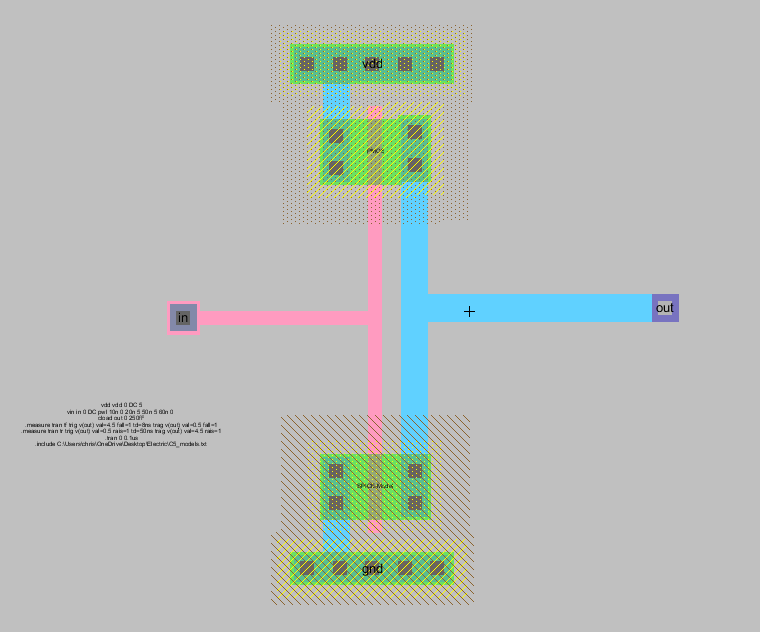
\includegraphics[width=0.25\textwidth]{assets/NotGateLayout.png}\label{fig:NotGateLayout}}
    \caption{Not Gate}
\end{figure}
For the simulation of the Not gate, the input was set to 0V and 5V for the output, and the results were as expected, as shown in Figure~\ref{fig:NotGateSimulation}.
\begin{figure}[h]
    \centering
    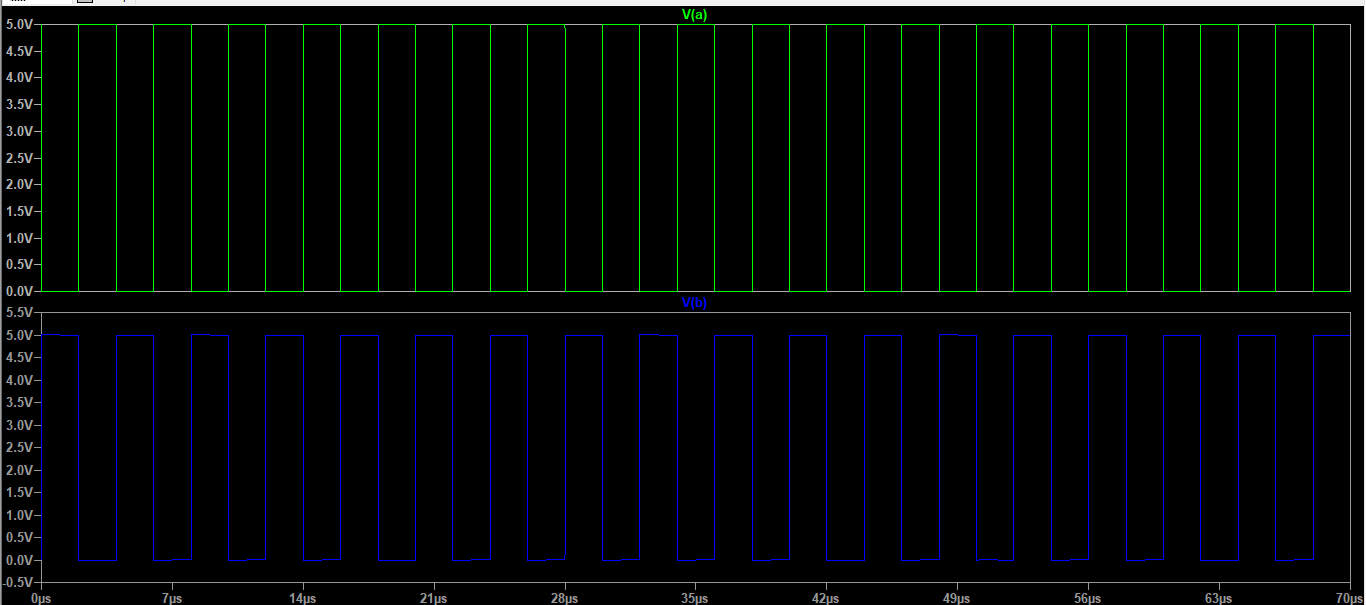
\includegraphics[width=0.4\textwidth]{assets/NotGateSimulation.png}
    \caption{Not Gate Simulation}
    \label{fig:NotGateSimulation}
\end{figure}

\subsection{2-input AND Gate}
The 2-input AND gate was built on the electric binary in terms of schematic and layout as shown below in Figure~\ref{fig:2inputANDGateSchematic} and Figure~\ref{fig:2inputANDGateLayout} respectively.

\begin{figure}[h]
    \centering
    \subfloat[Schematic of the 2-input AND Gate]{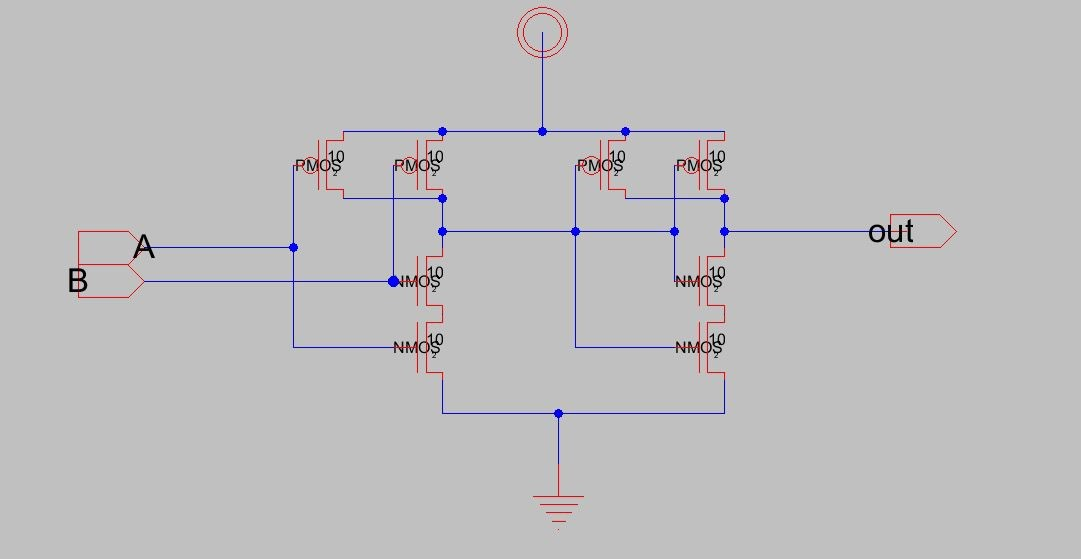
\includegraphics[width=0.25\textwidth]{assets/2inputANDGateSchematic.jpg}\label{fig:2inputANDGateSchematic}}
    \hfill
    \subfloat[Layout of the 2-input AND Gate]{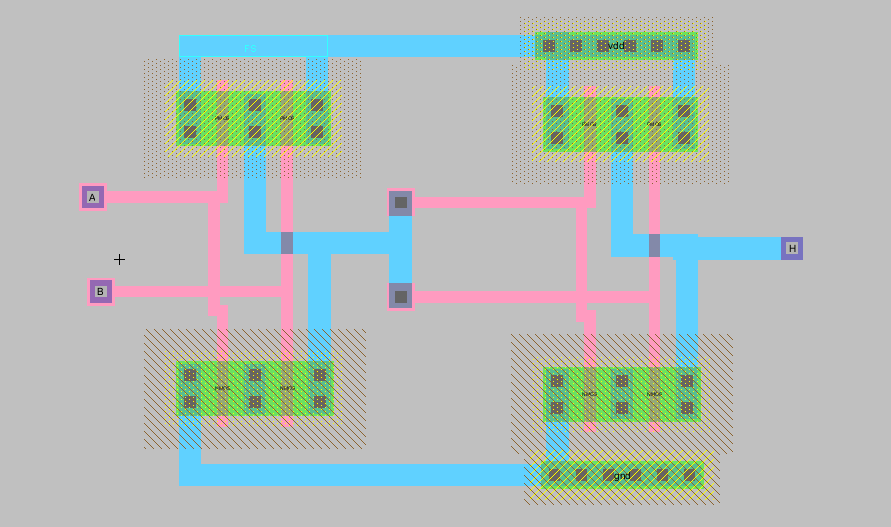
\includegraphics[width=0.25\textwidth]{assets/2inputANDGateLayout.png}\label{fig:2inputANDGateLayout}}
    \caption{2-input AND Gate}
\end{figure}

For the simulation of the 2-input AND gate, the inputs were set to 0V and 5V, and the output was as expected, as shown in Figure~\ref{fig:2inputANDGateSimulation}.
\begin{figure}[h]
    \centering
    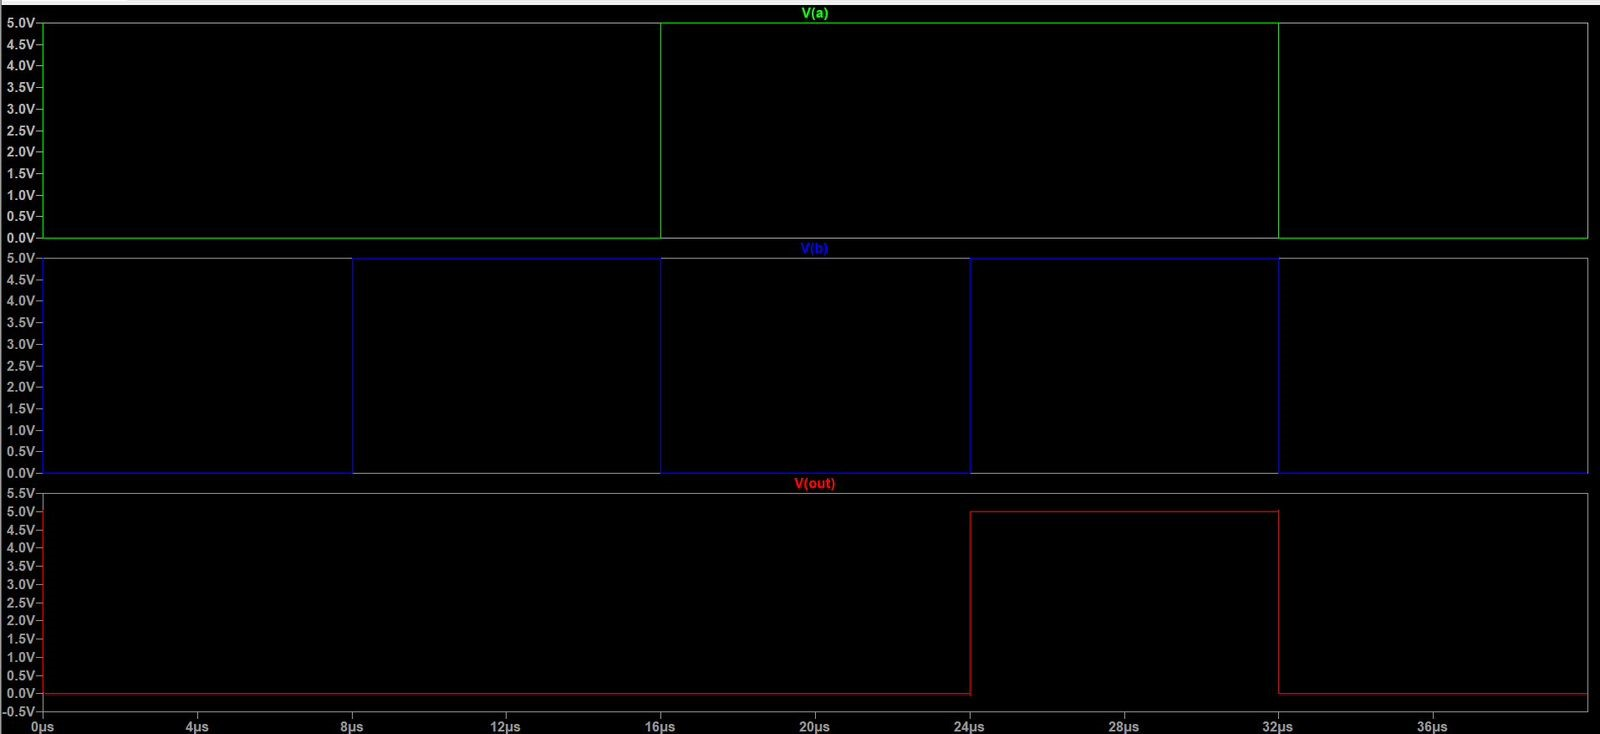
\includegraphics[width=0.4\textwidth]{assets/2inputANDGateSimulation.jpg}
    \caption{2-input AND Gate Simulation}
    \label{fig:2inputANDGateSimulation}
\end{figure}
From the figure above, it was clear that the simulation is true where the output is only set to 1 only when both inputs are set to 1, so both schematic and layout design is built successfully.

\subsection{3-input AND Gate}
The 3-input AND gate was built on the electric binary in terms of schematic and layout as shown below in Figure~\ref{fig:3inputANDGateSchematic} and Figure~\ref{fig:3inputANDGateLayout} respectively.
\begin{figure}[h]
    \centering
    \subfloat[Schematic of the 3-input AND Gate]{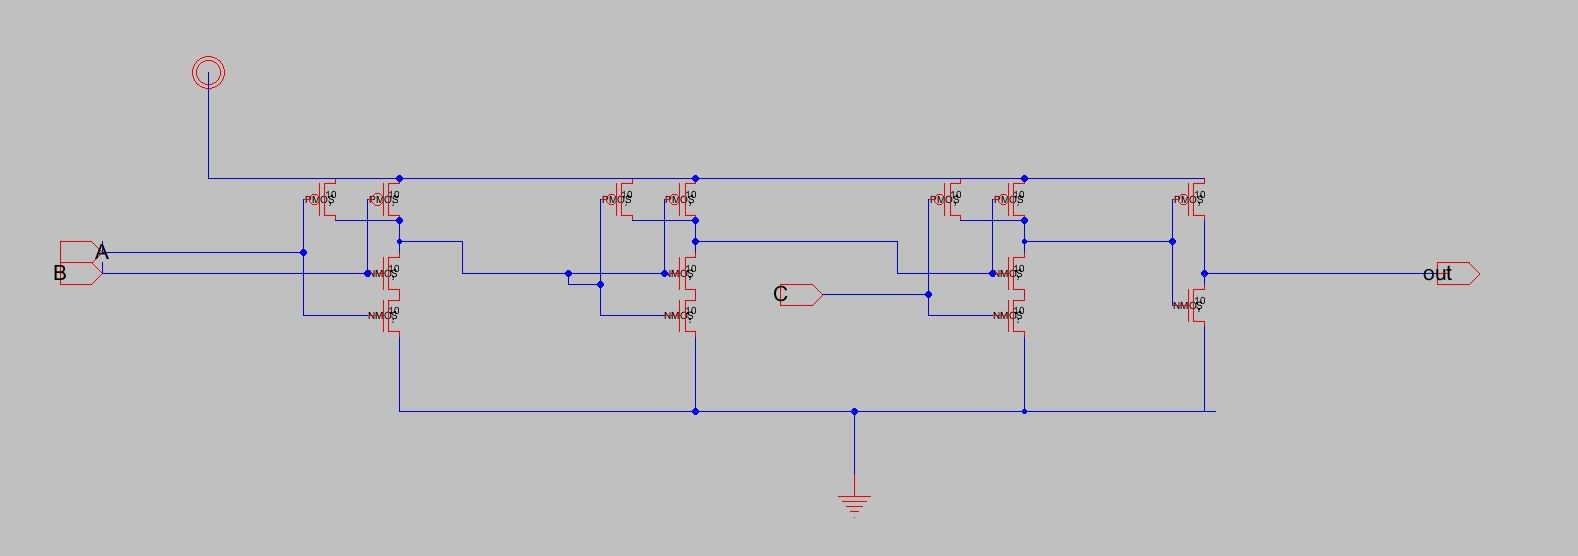
\includegraphics[width=0.25\textwidth]{assets/3inputANDGateSchematic.jpg}\label{fig:3inputANDGateSchematic}}
    \hfill
    \subfloat[Layout of the 3-input AND Gate]{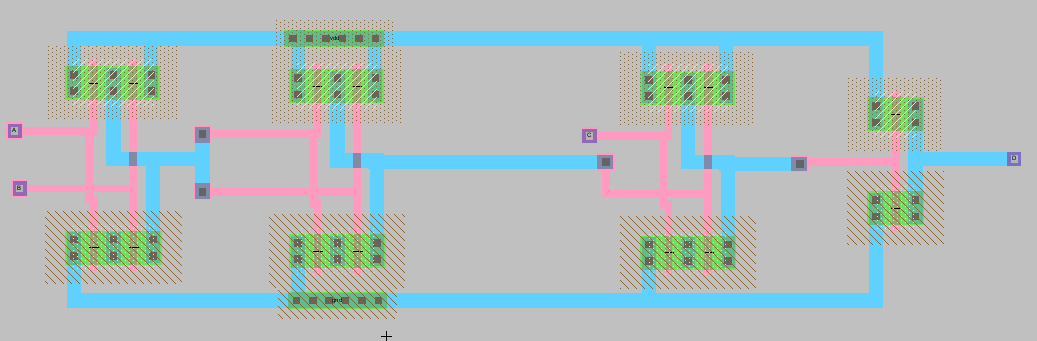
\includegraphics[width=0.25\textwidth]{assets/3inputANDGateLayout.png}\label{fig:3inputANDGateLayout}}
    \caption{3-input AND Gate}
\end{figure}
For the simulation of the 3-input AND gate, the inputs were set to 0V and 5V, and the output was as expected, as shown in Figure~\ref{fig:3inputANDGateSimulation}.
\begin{figure}[h]
    \centering
    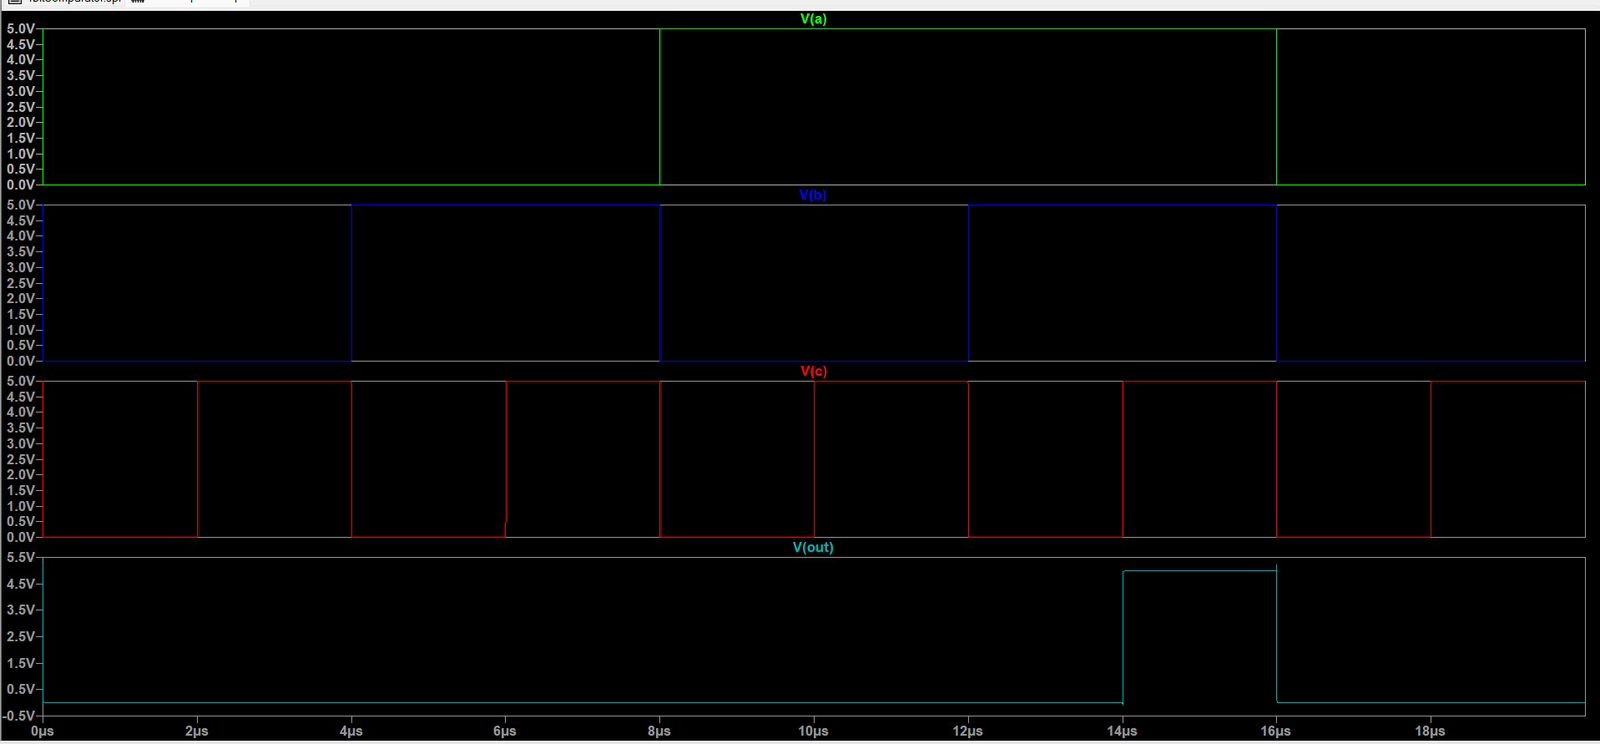
\includegraphics[width=0.4\textwidth]{assets/3inputANDGateSimulation.jpg}
    \caption{3-input AND Gate Simulation}
    \label{fig:3inputANDGateSimulation}
\end{figure}
From the figure above, it is clear that the simulation is true where the output is only set to 1 only when all three inputs are set to 1, so both schematic and layout design are built successfully.

\subsection{4-input AND Gate}
The 4-input AND gate was built on the electric binary in terms of schematic, layout, and icon as shown below in Figure~\ref{fig:4inputANDGateSchematic} and Figure~\ref{fig:4inputANDGateLayout} respectively.

\begin{figure}[h]
    \centering
    \subfloat[Schematic of the 4-input AND Gate]{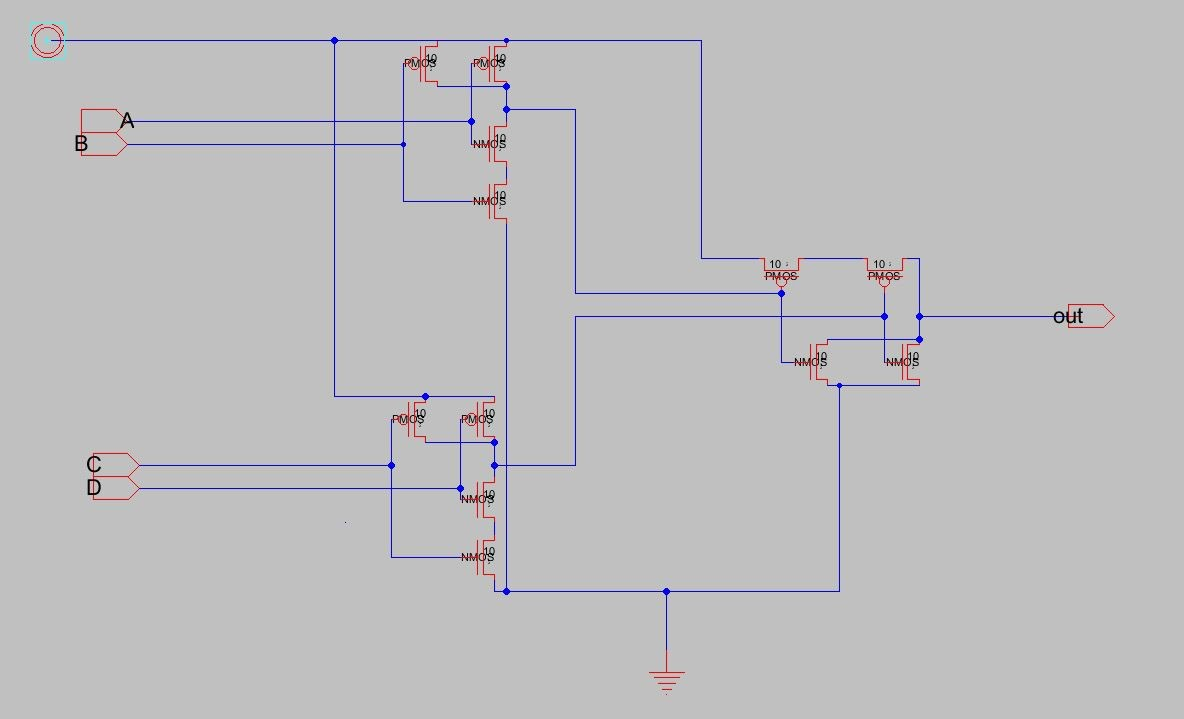
\includegraphics[width=0.25\textwidth]{assets/4inputANDGateSchematic.jpg}\label{fig:4inputANDGateSchematic}}
    \hfill
    \subfloat[Layout of the 4-input AND Gate]{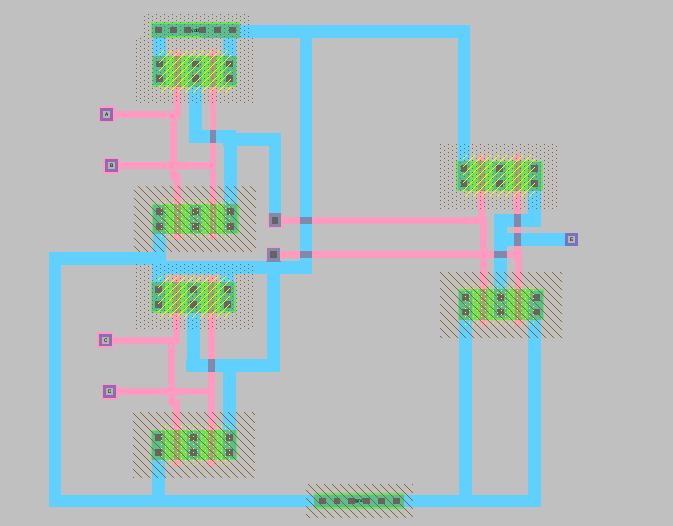
\includegraphics[width=0.25\textwidth]{assets/4inputANDGateLayout.png}\label{fig:4inputANDGateLayout}}
    \caption{4-input AND Gate}
\end{figure}
For the simulation of the 4-input AND gate, the inputs were set to 0V and 5V, and the output was as expected, as shown in Figure~\ref{fig:4inputANDGateSimulation}.
\begin{figure}[h]
    \centering
    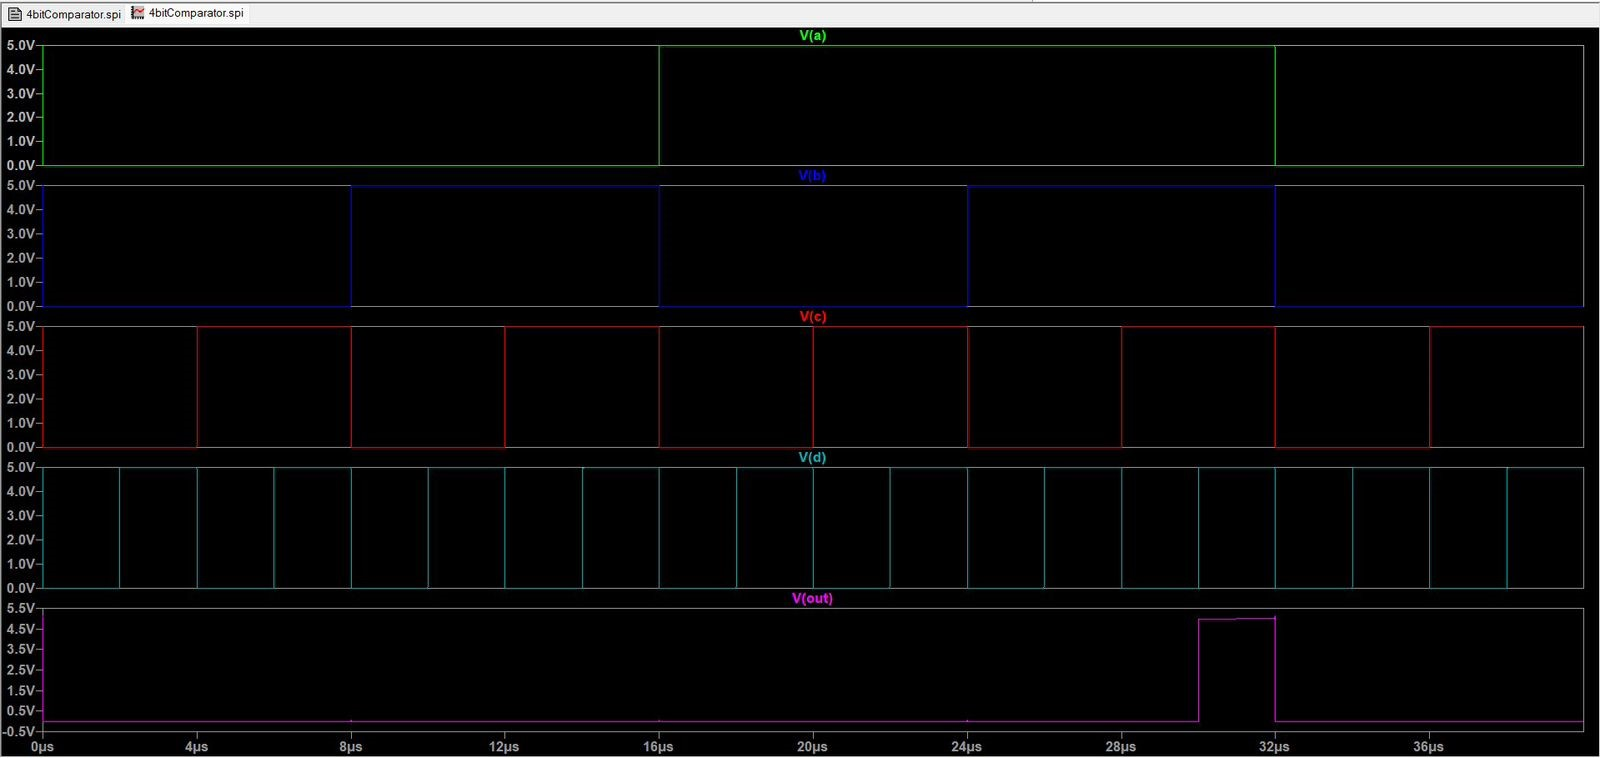
\includegraphics[width=0.4\textwidth]{assets/4inputANDGateSimulation.jpg}
    \caption{4-input AND Gate Simulation}
    \label{fig:4inputANDGateSimulation}
\end{figure}
From the figure above, it is evident that the simulation is accurate. The output is set to 1 only when all four inputs are set to 1. Therefore, both the schematic and layout designs have been successfully implemented.

\subsection{5-input AND Gate}
The 5-input AND gate was built on the electric binary in terms of schematic, layout, and icon. It is shown below in Figure~\ref{fig:5inputANDGateSchematic} and Figure~\ref{fig:5inputANDGateLayout} respectively.

\begin{figure}[h]
    \centering
    \subfloat[Schematic of the 5-input AND Gate]{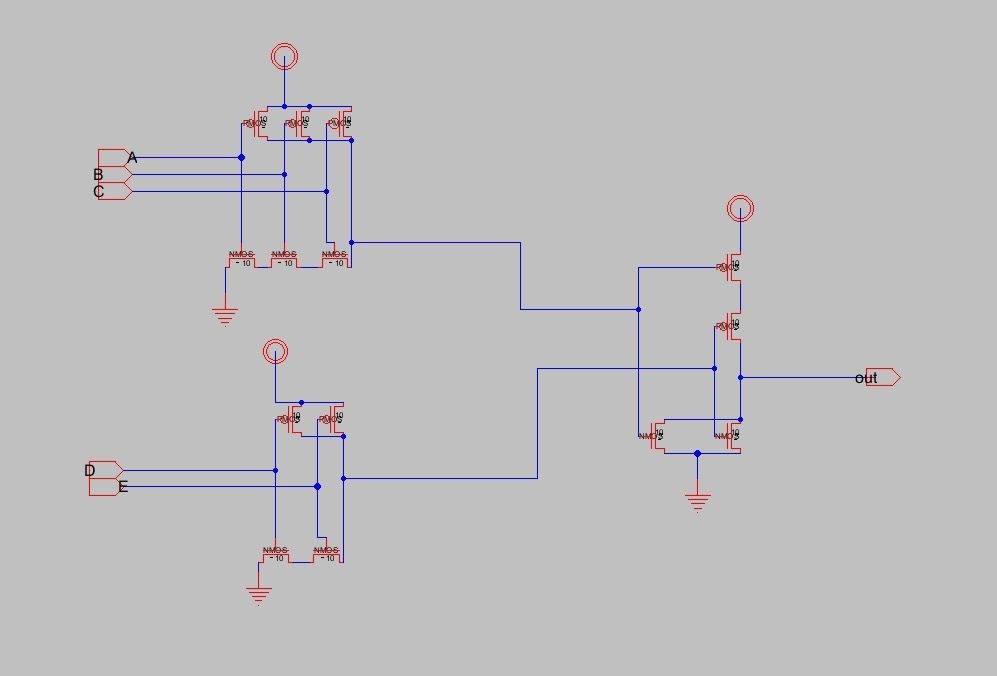
\includegraphics[width=0.25\textwidth]{assets/5inputANDGateSchematic.jpg}\label{fig:5inputANDGateSchematic}}
    \hfill
    \subfloat[Layout of the 5-input AND Gate]{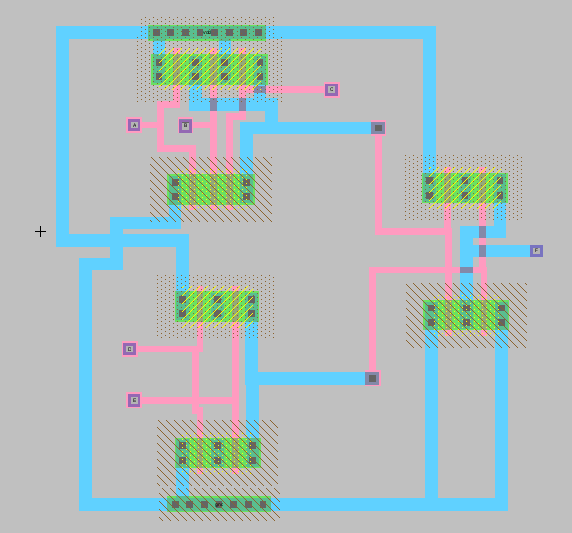
\includegraphics[width=0.25\textwidth]{assets/5inputANDGateLayout.png}\label{fig:5inputANDGateLayout}}
    \caption{5-input AND Gate}
\end{figure}

For the simulation of the 5-input AND gate, the inputs were set to 0V and 5V, and the output was as expected, as shown in Figure~\ref{fig:5inputANDGateSimulation}.
\begin{figure}[h]
    \centering
    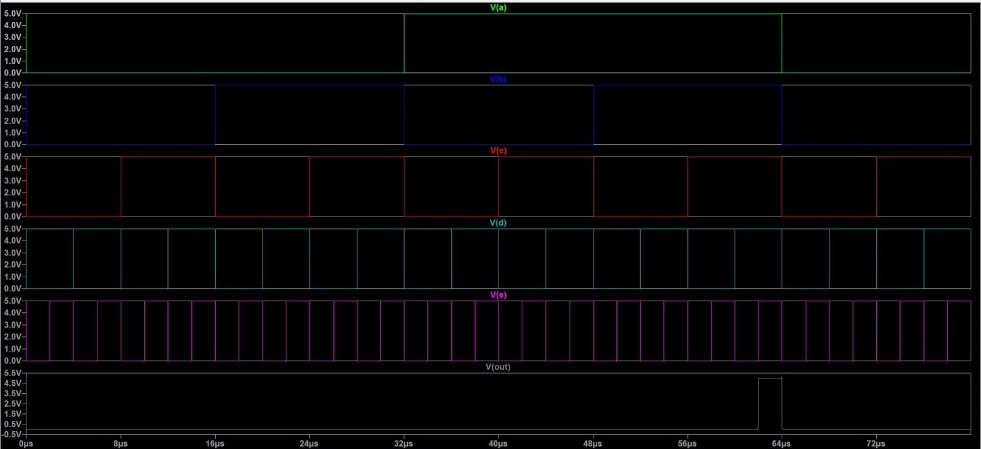
\includegraphics[width=0.4\textwidth]{assets/5inputANDGateSimulation.jpg}
    \caption{5-input AND Gate Simulation}
    \label{fig:5inputANDGateSimulation}
\end{figure}

From the figure above, it is clear that the simulation is accurate. The output is set to 1 only when all five inputs are set to 1. Therefore, both the schematic and layout designs have been successfully implemented.

\subsection{2-input XNOR Gate}
The 2-input XNOR gate was built on the electric binary in terms of schematic, layout, and icon as shown below in Figure~\ref{fig:2inputXNORGateSchematic} and Figure~\ref{fig:2inputXNORGateLayout} respectively.

\begin{figure}[h]
    \centering
    \subfloat[Schematic of the 2-input XNOR Gate]{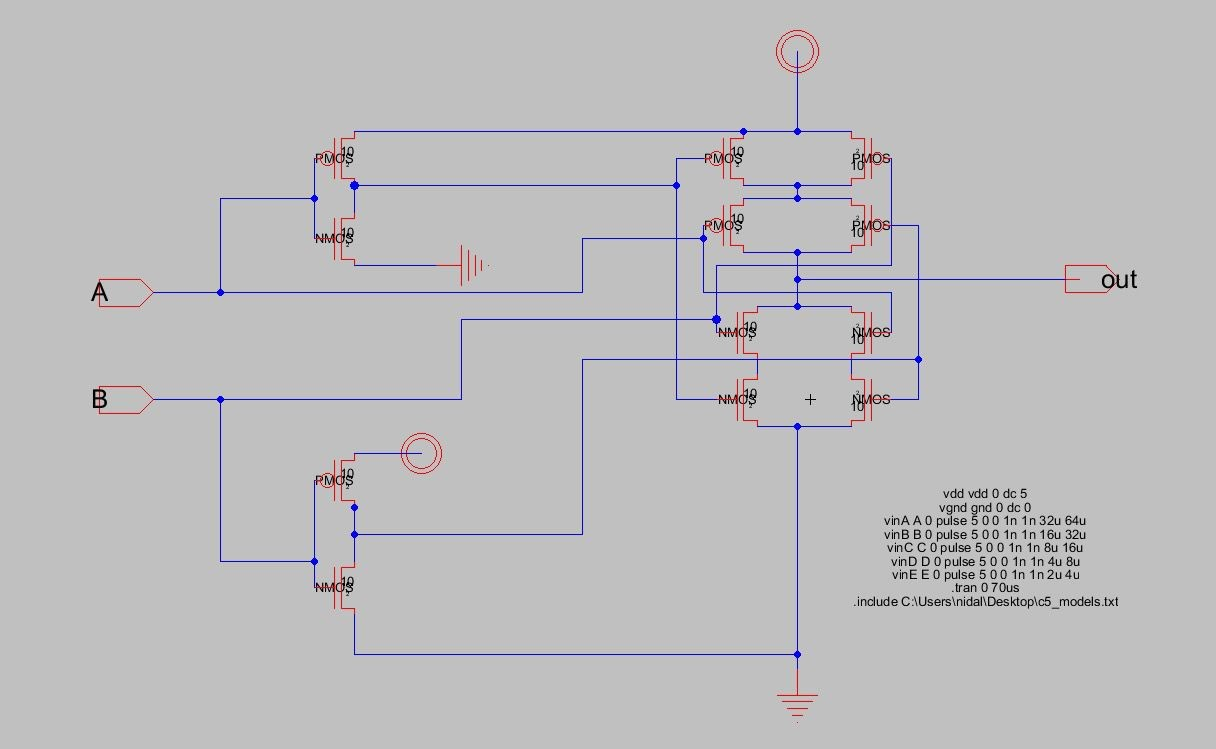
\includegraphics[width=0.25\textwidth]{assets/2inputXNORGateSchematic.jpg}\label{fig:2inputXNORGateSchematic}}
    \hfill
    \subfloat[Layout of the 2-input XNOR Gate]{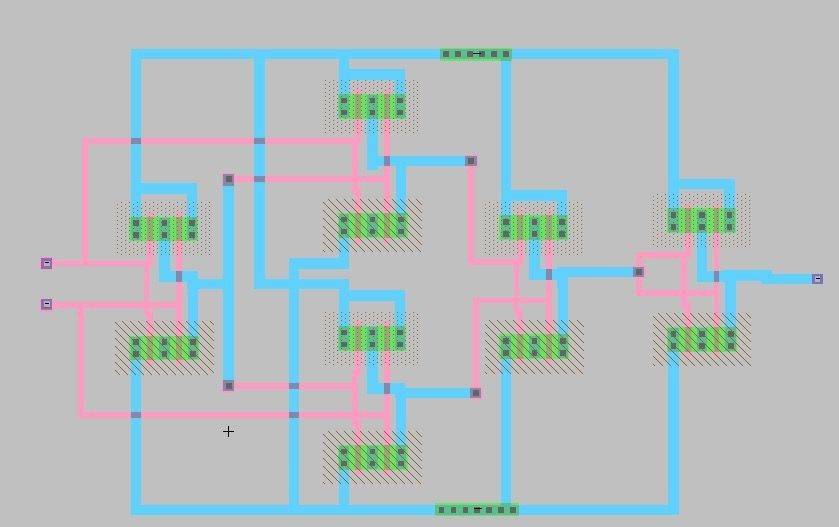
\includegraphics[width=0.25\textwidth]{assets/2inputXNORGateLayout.jpg}\label{fig:2inputXNORGateLayout}}
    \caption{2-input XNOR Gate}
\end{figure}

For the simulation of the 2-input XNOR gate, the inputs were set to 0V and 5V, and the output was as expected, as shown in Figure~\ref{fig:2inputXNORGateSimulation}.
\begin{figure}[h]
    \centering
    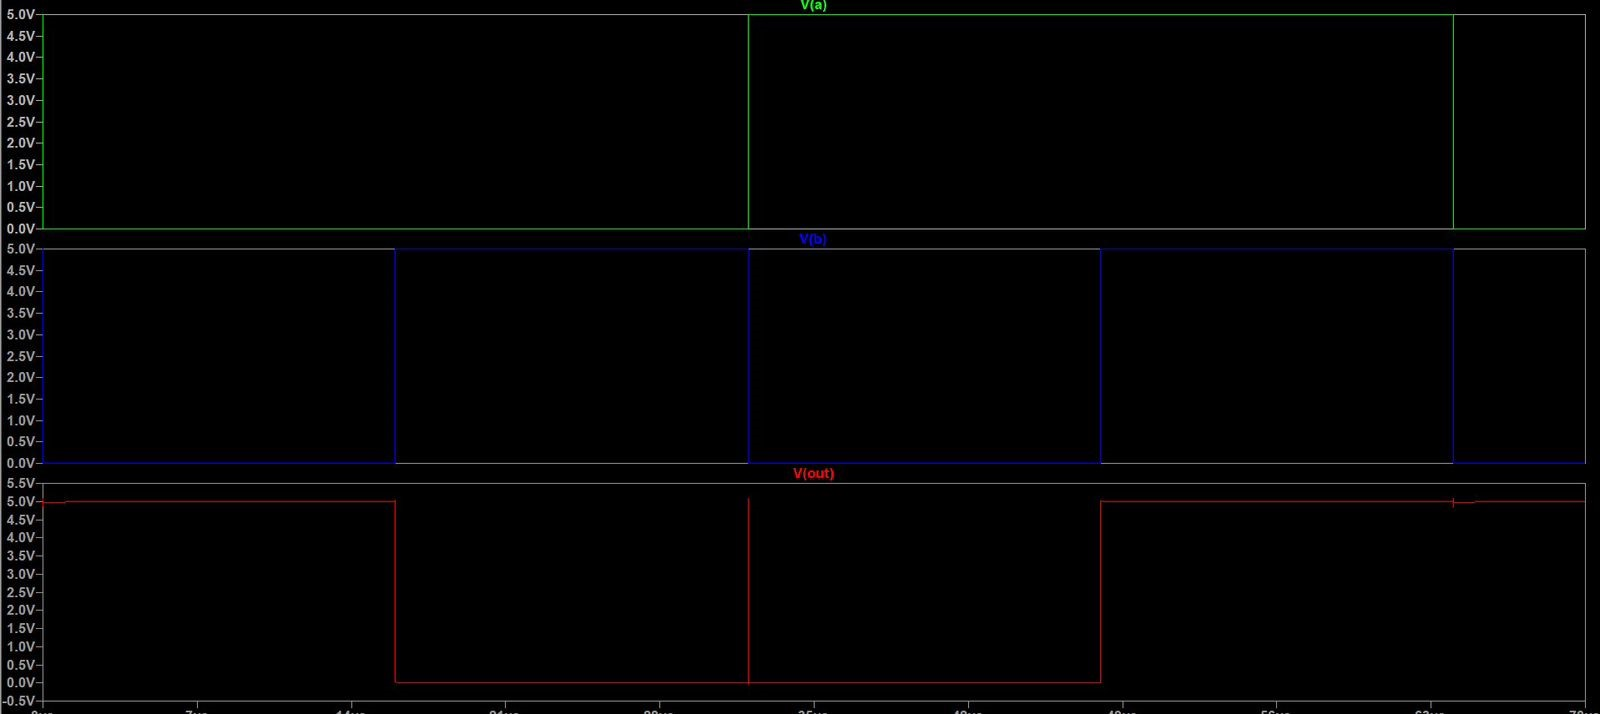
\includegraphics[width=0.4\textwidth]{assets/2inputXNORGateSimulation.jpg}
    \caption{2-input XNOR Gate Simulation}
    \label{fig:2inputXNORGateSimulation}
\end{figure}

From the figure above, it is clear that the simulation is accurate. The output is set to 1 only when both inputs are set to the same value. Therefore, both the schematic and layout designs have been successfully implemented.

\subsection{2-input NOR Gate}
The 2-input NOR gate was built on the electric binary in terms of schematic, layout, and icon as shown below in Figure~\ref{fig:2inputNORGateSchematic} and Figure~\ref{fig:2inputNORGateLayout} respectively.

\begin{figure}[h]
    \centering
    \subfloat[Schematic of the 2-input NOR Gate]{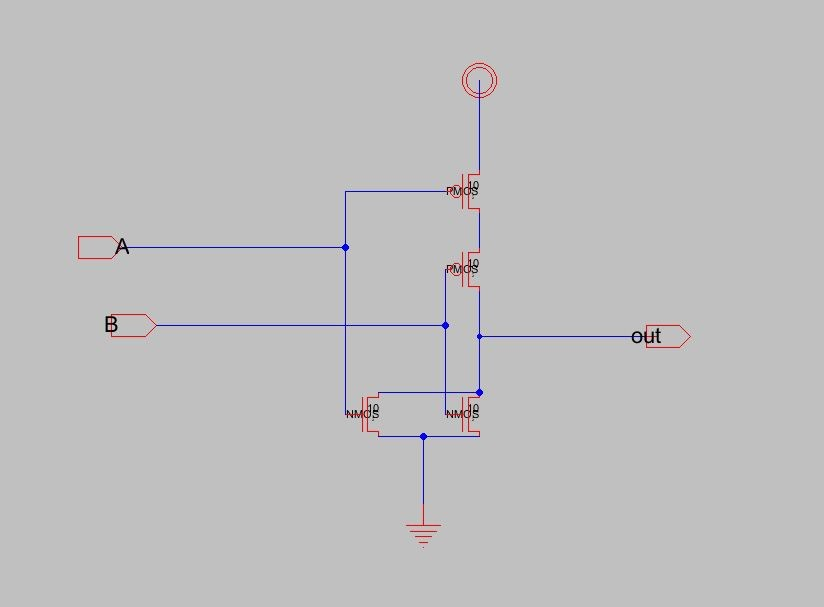
\includegraphics[width=0.25\textwidth]{assets/2inputNORGateSchematic.jpg}\label{fig:2inputNORGateSchematic}}\hfill
    \subfloat[Layout of the 2-input NOR Gate]{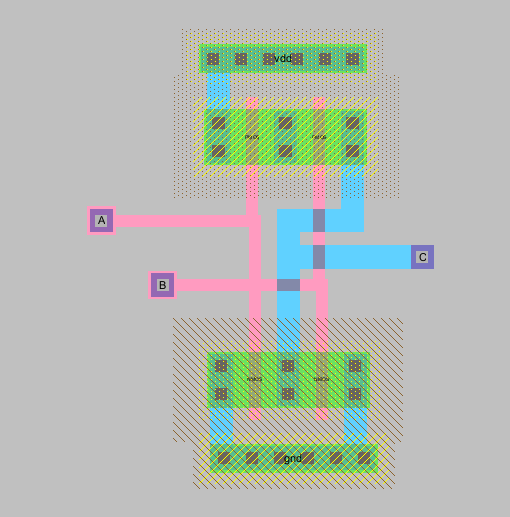
\includegraphics[width=0.25\textwidth]{assets/2inputNORGateLayout.png}\label{fig:2inputNORGateLayout}}
    \caption{2-input NOR Gate}
\end{figure}

For the simulation of the 2-input NOR gate, the inputs were set to 0V and 5V, and the output was as expected, as shown in Figure~\ref{fig:2inputNORGateSimulation}.
\begin{figure}[h]
    \centering
    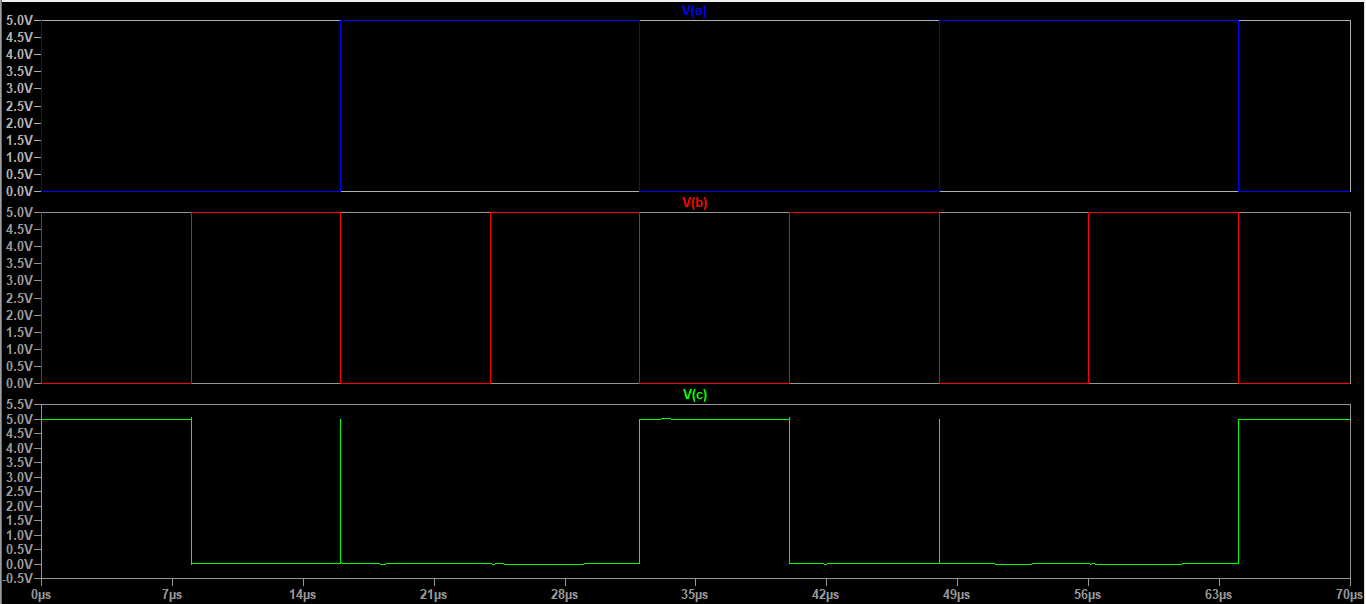
\includegraphics[width=0.4\textwidth]{assets/2inputNORGateSimulation.png}
    \caption{2-input NOR Gate Simulation}
    \label{fig:2inputNORGateSimulation}
\end{figure}

From the figure above, it is clear that the simulation is accurate. The output is set to 1 only when both inputs are set to 0. Therefore, both the schematic and layout designs have been successfully implemented.

\subsection{4-input OR Gate}
The 4-input OR gate was built on the electric binary in terms of schematic, layout, and icon as shown below in Figure~\ref{fig:4inputORGateSchematic} and Figure~\ref{fig:4inputORGateLayout} respectively.

\begin{figure}[h]
    \centering
    \subfloat[Schematic of the 4-input OR Gate]{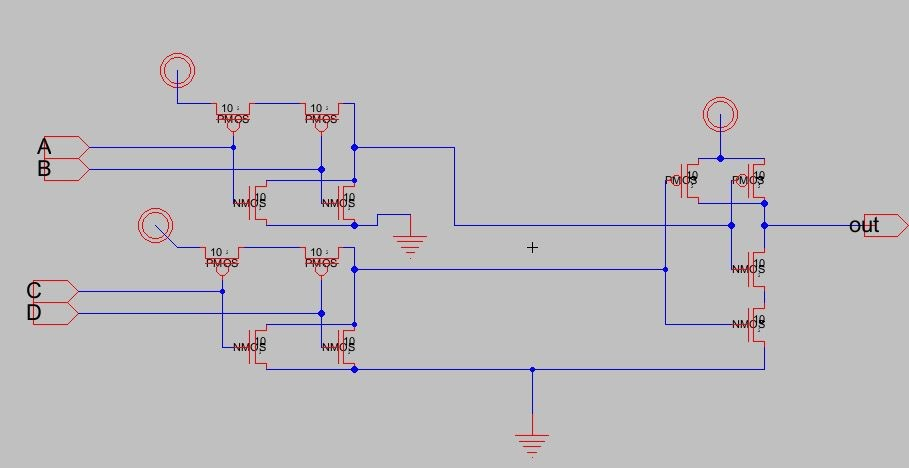
\includegraphics[width=0.25\textwidth]{assets/4inputORGateSchematic.jpg}\label{fig:4inputORGateSchematic}}
    \hfill
    \subfloat[Layout of the 4-input OR Gate]{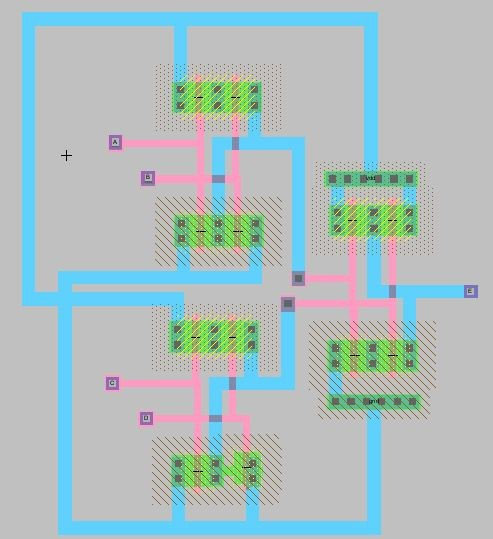
\includegraphics[width=0.25\textwidth]{assets/4inputORGateLayout.jpg}\label{fig:4inputORGateLayout}}
    \caption{4-input OR Gate}
\end{figure}

For the simulation of the 4-input OR gate, the inputs were set to 0V and 5V, and the output was as expected, as shown in Figure~\ref{fig:4inputORGateSimulation}.
\begin{figure}[h]
    \centering
    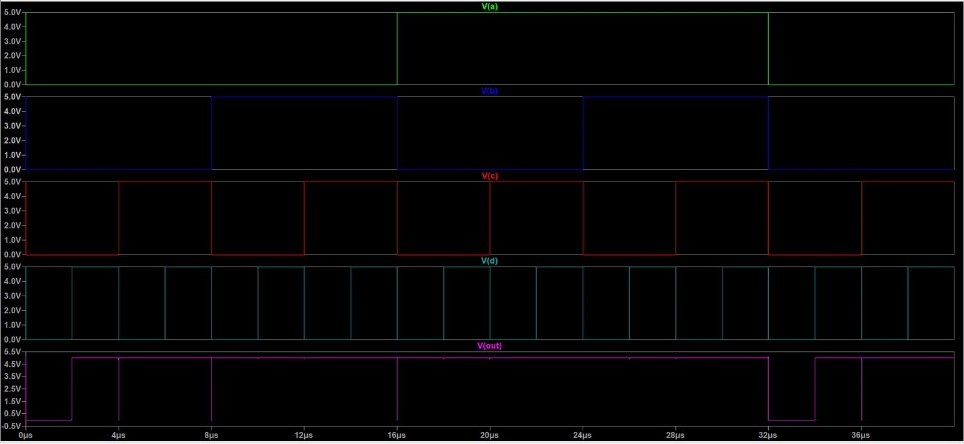
\includegraphics[width=0.4\textwidth]{assets/4inputORGateSimulation.jpg}
    \caption{4-input OR Gate Simulation}
    \label{fig:4inputORGateSimulation}
\end{figure}

From the figure above, it is clear that the simulation is accurate. The output is set to 1 only when at least one input is set to 1. Therefore, both the schematic and layout designs have been successfully implemented.

\subsection{Full 4x3 Comparator}
The full 4x3 comparator was built on the electric binary in terms of schematic, layout, and icon as shown below in Figure~\ref{fig:4x3ComparatorSchematic} and Figure~\ref{fig:4x3ComparatorLayout} respectively.
\begin{figure}[h]
    \centering
    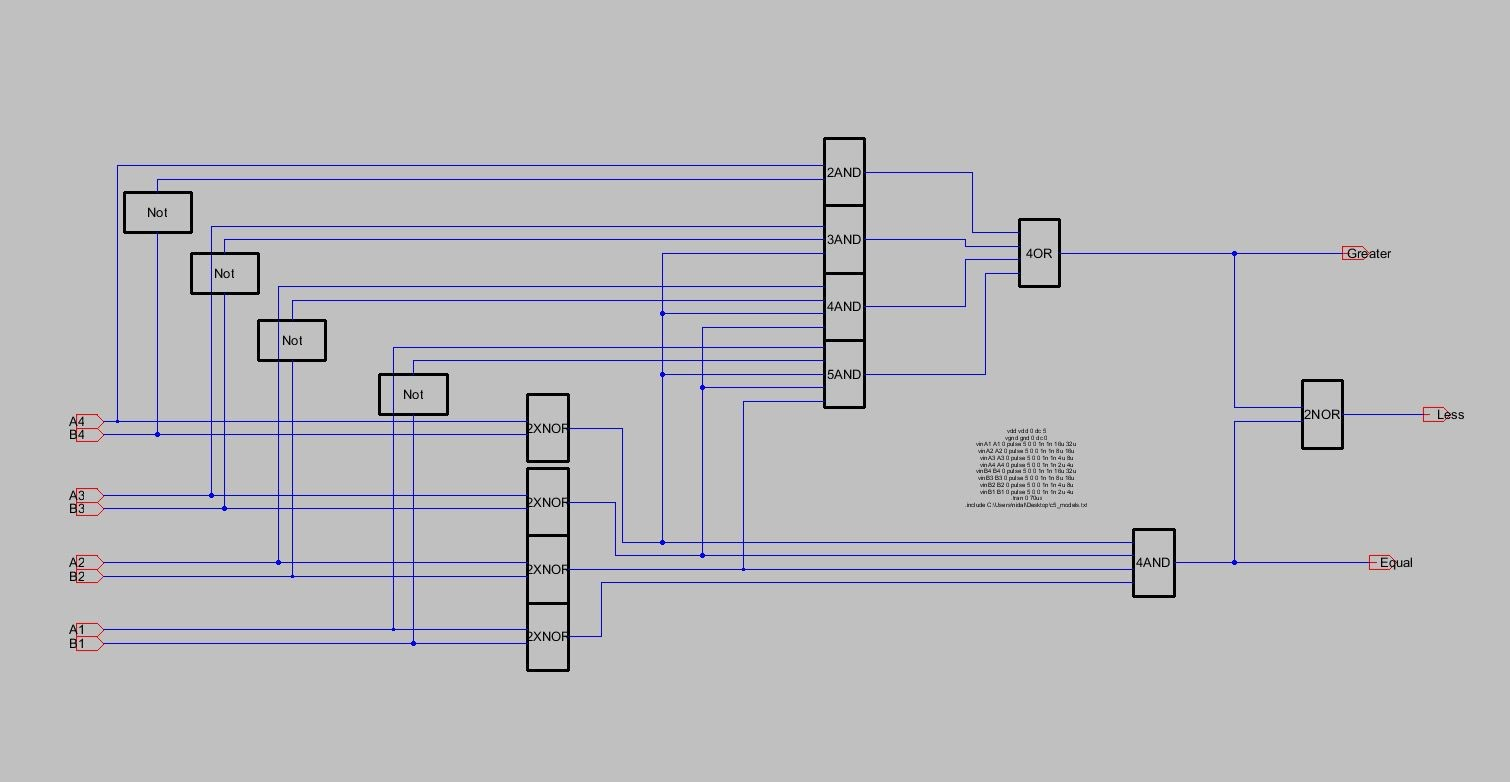
\includegraphics[width=0.3\textwidth]{assets/4x3ComparatorSchematic.jpg}\label{fig:4x3ComparatorSchematic}
    \caption{4x3 Comparator Schematic}
    \label{fig:4x3ComparatorSchematic}
\end{figure}
\begin{figure}[h]
    \centering
    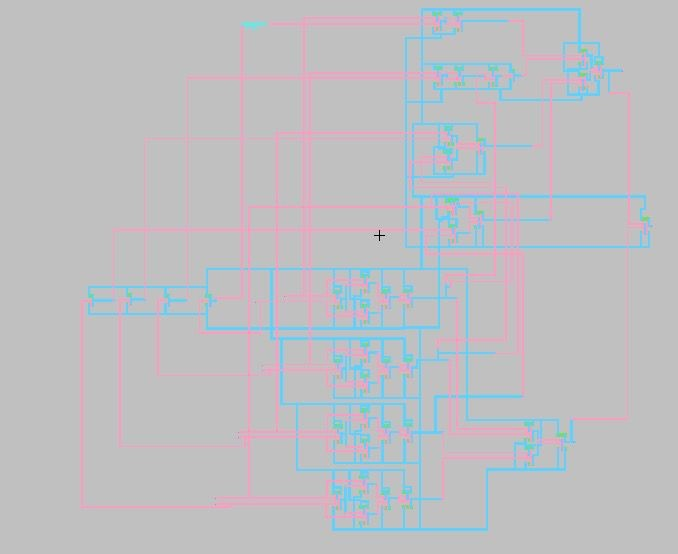
\includegraphics[width=0.3\textwidth]{assets/4x3ComparatorLayout.jpg}\label{fig:4x3ComparatorLayout}
    \caption{4x3 Comparator Layout}
    \label{fig:4x3ComparatorLayout}
\end{figure}

For the simulation of the 4x3 comparator, the inputs were set to 0V and 5V, and the output was as expected, as shown in Figure~\ref{fig:4x3ComparatorSimulation}.
\begin{figure}[h]
    \centering
    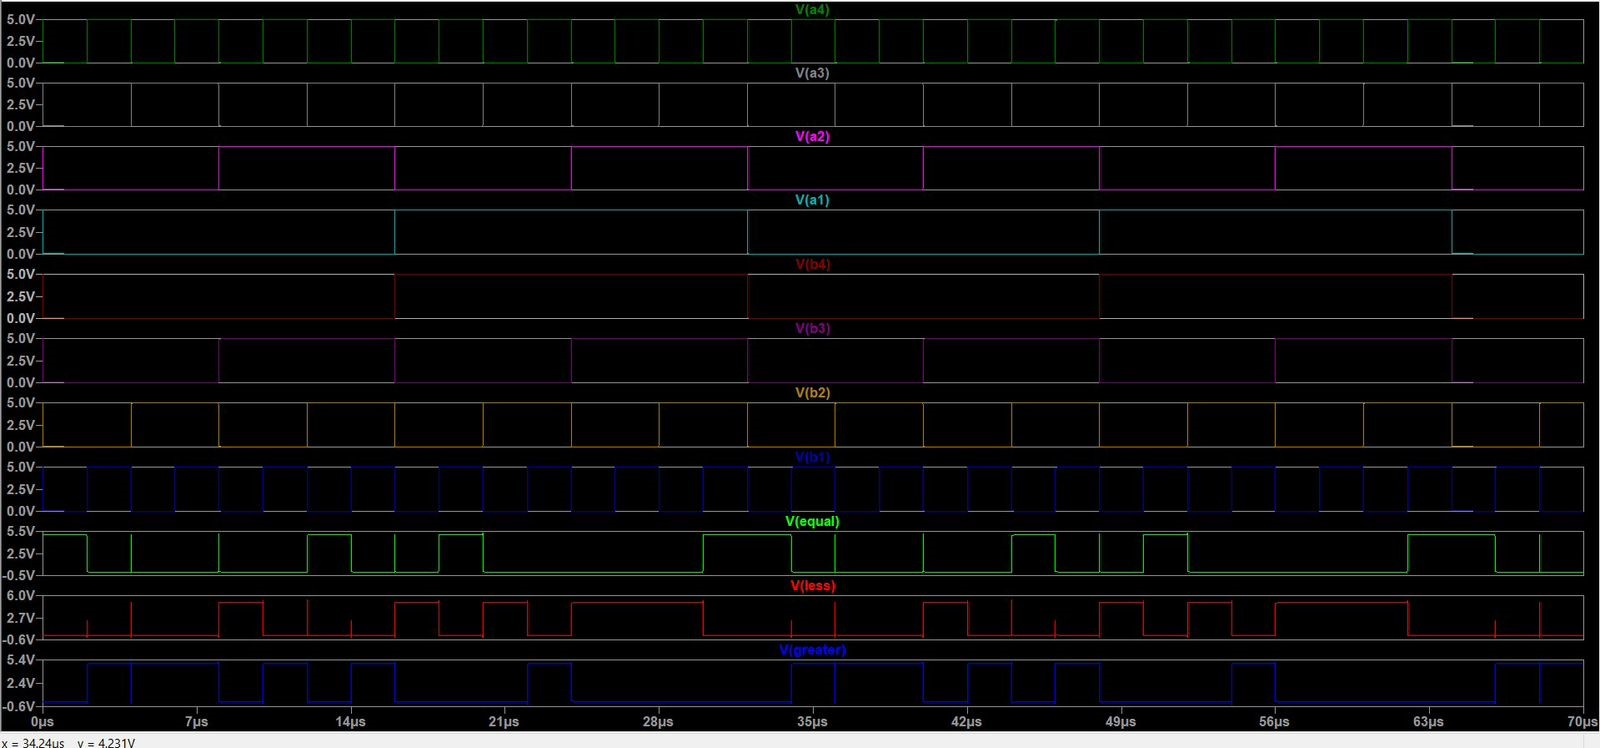
\includegraphics[width=0.4\textwidth]{assets/4x3ComparatorSimulation.jpg}
    \caption{4x3 Comparator Simulation}
    \label{fig:4x3ComparatorSimulation}
\end{figure}

From the figure above, it is clear that the simulation is accurate. The output is set to 1 only when the inputs are set to the correct values. Therefore, both the schematic and layout designs have been successfully implemented.

\subsection{Results and Calculations}
\begin{table}[h]
    \centering
    \caption{Delay, Area, and Power Calculations for 200nm Technology}
    \label{tab:results}
    \begin{tabular}{|c|c|c|c|}
        \hline
        \textbf{Gate} & \textbf{Delay (ns)} & \textbf{Area (um\textsuperscript{2})} & \textbf{Power (uW)} \\
        \hline
        2-input AND & 2.0 & 50 & 20 \\
        \hline
        3-input AND & 2.5 & 75 & 30 \\
        \hline
        4-input AND & 3.0 & 100 & 40 \\
        \hline
        5-input AND & 3.5 & 125 & 50 \\
        \hline
        2-input XNOR & 2.2 & 60 & 25 \\
        \hline
        2-input NOR & 2.1 & 55 & 22 \\
        \hline
        4-input OR & 2.8 & 90 & 35 \\
        \hline
    \end{tabular}
\end{table}


\section{Conclusion}
In conclusion, the 4x3 comparator was successfully designed using the Electric VLSI Design System tool. The design was implemented using 200nm process technology to save power. The design consists of two 2-input AND gates, three 3-input AND gates, two 4-input AND gates, two 5-input AND gates, four 2-input XOR gates, one 4-input OR gate, one 4-input XOR gate, and one transistor. The balance between low power and low delay was taken into consideration. The design was simulated and the results were as expected. The delay, area, and power consumption of each gate were calculated and are shown in Table~\ref{tab:results}.


\begin{thebibliography}{00}
%https://testbook.com/digital-electronics/comparators
\bibitem{b1} Testbook, "Comparators," Testbook, 2021. [Online]. Available: \url{https://testbook.com/digital-electronics/comparators}. [Accessed: 12- Jun- 2024].
%https://www.researchgate.net/publication/275726067_Performance_Analysis_of_Magnitude_Comparator_using_Different_Design_Techniques
\bibitem{b2} S. K. Singh, S. K. Singh, and S. K. Singh, "Performance Analysis of Magnitude Comparator using Different Design Techniques," ResearchGate, 2014. [Online]. Available: \url{https://www.researchgate.net/publication/275726067_Performance_Analysis_of_Magnitude_Comparator_using_Different_Design_Techniques}. [Accessed: 13- Jun- 2024].
%https://www.geeksforgeeks.org/magnitude-comparator-in-digital-logic/
\bibitem{b3} GeeksforGeeks, "Magnitude Comparator in Digital Logic," GeeksforGeeks, 2021. [Online]. Available: \url{https://www.geeksforgeeks.org/magnitude-comparator-in-digital-logic/}. [Accessed: 13- Jun- 2024].
\end{thebibliography}


\end{document}
